%%%%%%%%%%%%%%%%%%%%%%%%%%%%%%%%%%%%%%%%%%%%%%
%                insertmeeting
% 1) Title (something creative & funny?)
% 2) Date (MM/DD/YYYY)
% 3) Location (ex. Hagerty High School)
% 4) People/Committees Present 
% 5) Picture 
% 6) Start Time & Stop Time (ex. 12:30AM to 4:30PM)
%%%%%%%%%%%%%%%%%%%%%%%%%%%%%%%%%%%%%%%%%%%%%%
\insertmeeting 
	{Kalman Kangarooing} 
	{04/07/22} 
	{Hagerty High School}
	{James, Jensen, Nathan, Ritam}
	{Images/RobotPics/robot.jpg}
	{2:30 - 4:30}
	
\hhscommittee{Software}
\noindent\hfil\rule{\textwidth}{.4pt}\hfil
\subsubsection*{Goals}
\begin{itemize}
    \item Explore the possibility of using a Kalman filter.

\end{itemize} 

\noindent\hfil\rule{\textwidth}{.4pt}\hfil

\subsubsection*{Accomplishments}
One possibility raised at the meeting with our mentor today was possible introduction of a Kalman filter into our code. Essentially the Kalman filter reduces the noise of sensor data using a prediction and correction stage. The prediction looks at what we expected the reading to be, then measured the actual value. Using this difference, it adjusts its next prediction. Eventually, this prediction should come much closer to the true value than all of the actual sensor readings, which could be incorrect. While this was the approach created by TRC, we quickly realized that their implementation would only work for a single sensor. Our goal was to fuse the heading from kinematics and gyro heading to find a better value for our robot's true heading. However, this seemed really complex. There's a lot of math involved with matrices and probability that our members had not yet been exposed to. While we were able to understand the Kalman filter on a very abstract level, it seemed extremely difficult to implement. Just like the brake mode from last week, it didn't seem to be the most effective use of our remaining time to implement such a complicated system. Because our current localization system relying on the REV Hub's IMU was working well enough, we decided once again that our time would best be spent refining the autonomous program for consistency and driver practice. 


\begin{figure}[htp]
\centering
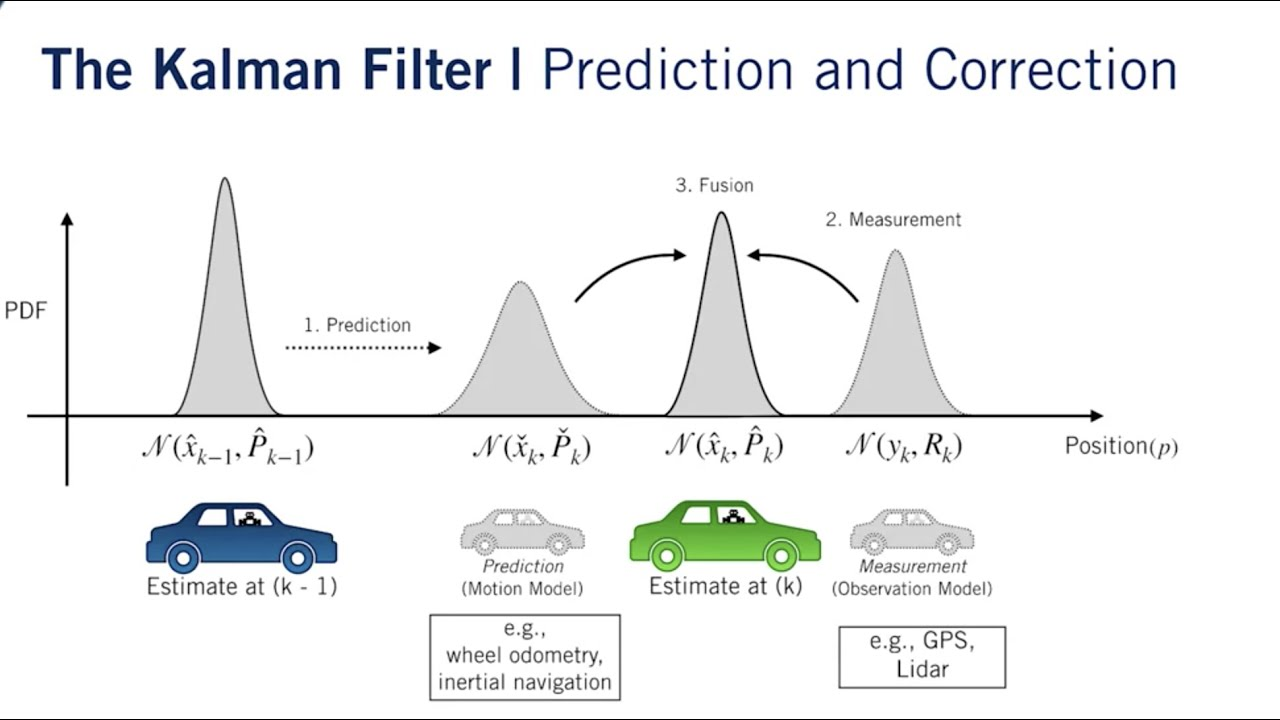
\includegraphics[width=0.95\textwidth, angle=0]{Meetings/April/04-07-22/04-07-22 1.JPG}
\caption{Infographic summarizing the Kalman filter.}
\label{fig:040722_1}
\end{figure}

\begin{figure}[htp]
\centering
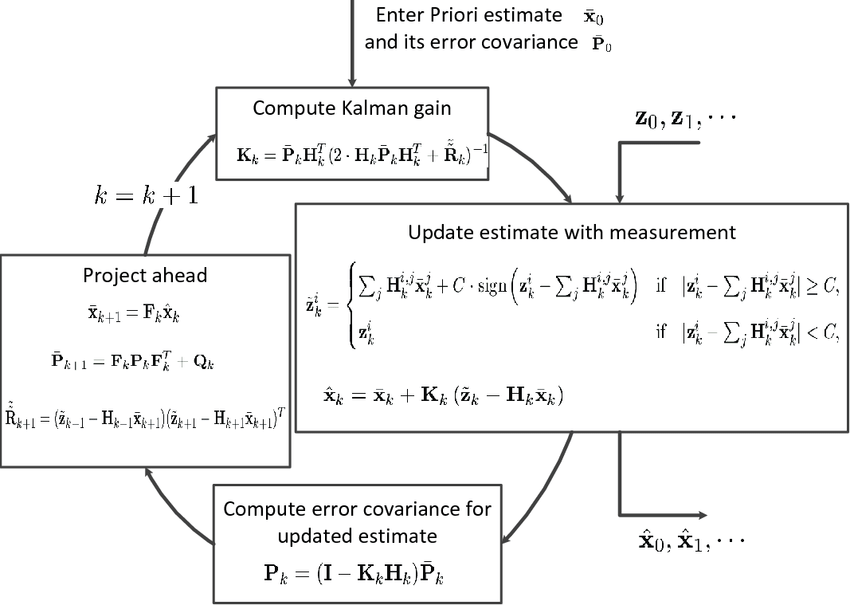
\includegraphics[width=0.95\textwidth, angle=0]{Meetings/April/04-07-22/04-07-22 2.png}
\caption{A more detailed explanation of the Kalman filter. While the high level concepts of prediction and correction made sense, many of the mathematicl equations were above our level.}
\label{fig:040722_2}
\end{figure}

\begin{figure}[htp]
\centering
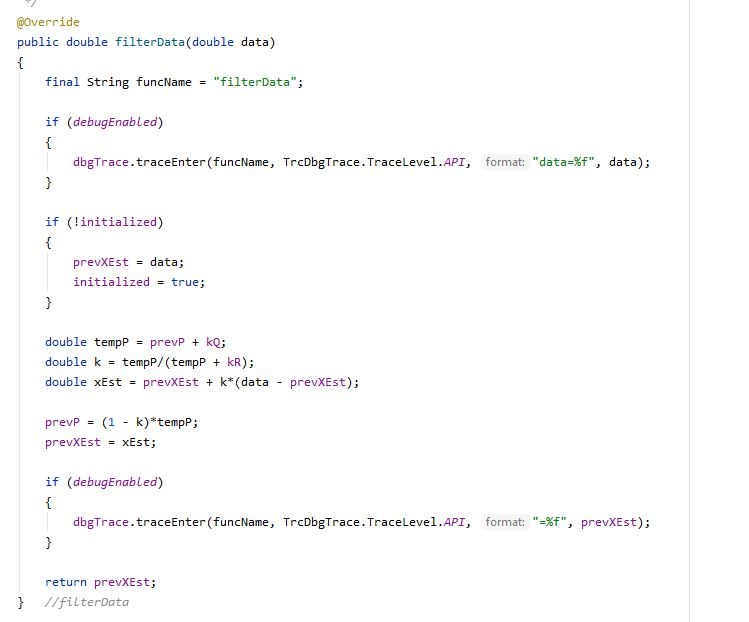
\includegraphics[width=0.95\textwidth, angle=0]{Meetings/April/04-07-22/04-07-22 3.JPG}
\caption{TRC's provided single-sensor Kalman filter.}
\label{fig:040722_3}
\end{figure}



\whatsnext{
\begin{itemize}
    \item Prepare the autonomous program for Worlds.
\end{itemize} 
}

